\section{Redes de Petri Temporales}
	
	En los modelos de Redes de Petri descriptos hasta el momento, el tiempo no estaba considerado. 
	
	En el formalismo de Redes de Petri b�sico, o aut�nomo, la abstracci�n del entorno en el que la red 
	evoluciona, incluyendo el tiempo como parte de este entorno, es total. Por lo que existe cierto 
	indeterminismo en cuanto al tiempo: no se especifica cu�ndo se disparar� una transici�n que est� 
	sensibilizada (ni si se disparar� realmente), tampoco cu�l de entre un grupo de transiciones en conflicto 
	ser� la disparada \cite{garciaizquierdo}.
	
	Las distintas interpretaciones con tiempo de las Redes de Petri han tratado de reducir el indeterminismo 
	de distintas maneras. Entre estas interpretaciones est�n:
	\begin{enumerate}
	  	\renewcommand{\theenumi}{\Alph{enumi}}
	  	\item \underline{Redes de Petri Estoc�sticas (Stochastic Petri Net)}
	  		\\
			Se introduce una estimaci�n estoc�stica respecto del instante de disparo de una transici�n.
		\item \underline{Redes de Petri Temporizadas (Timed Petri Net)}
			\\
			Introduce una condici�n de tiempo que establece la duraci�n de la transici�n.
		\item \underline{Redes de Petri con Tiempo (Time Petri Net)}
			\\
			Introducen cotas temporales entre las cuales la transici�n puede o debe ser disparada.
	\end{enumerate}
	
	\begin{figure}[ht]
		\centering
		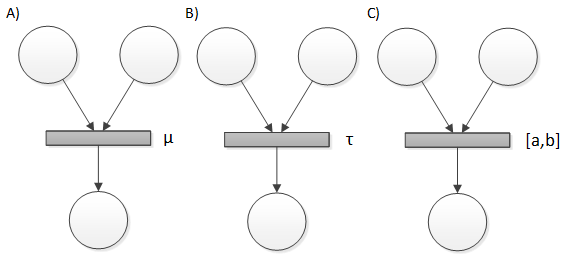
\includegraphics[width=1\linewidth]{Petri16}
		\caption{Interpretaciones de Redes de Petri Temporales}
		\label{fig:Petri16}
	\end{figure}
 
	Existen dos maneras de interpretar el par�metro temporal asociado a una transici�n:
	\begin{itemize}
		\item Cuando el par�metro temporal determina el tiempo que ha de transcurrir desde que una transici�n 
			queda sensibilizada hasta que se dispara, procedi�ndose entonces a la retirada y colocaci�n de marcas 
			de forma at�mica, se habla de \textbf{\emph{tiempo de sensibilizaci�n (enabling time)}}.
			Est� relacionada con las \textbf{\emph{Redes de Petri con Tiempo}} (Red C de la figura \ref{fig:Petri16}).
		
		\item El par�metro temporal puede determinar tambi�n el tiempo que debe transcurrir entre la retirada 
			(instant�nea) de marcas de los lugares de entrada, y la colocaci�n (instant�nea) de marcas en los 
			lugares de salida; en este caso se habla de tiempo de \textbf{\emph{disparo (firing time)}}.
			Esto es, el disparo de la transici�n tiene tres fases (retirada de marcas de entrada, disparo, 
			colocaci�n de marcas de salida) y no es at�mico, sino que tienen una duraci�n. Por ello esta 
			interpretaci�n es tambi�n conocida como sem�ntica de duraci�n.
		 
		Est�n asociadas con las \textbf{\emph{Redes de Petri Temporizadas}} (Red B de la figura \ref{fig:Petri16}).
	\end{itemize}